\documentclass[epsfig,10pt,fullpage]{article}

\newcommand{\LabNum}{1}
\newcommand{\CommonDocsPath}{../../../../common/docs}
\input{\CommonDocsPath/preamble.tex}

\begin{document}

\centerline{\huge Computer Organization}
~\\
\centerline{\huge Laboratory Exercise \LabNum}
~\\
\centerline{\large Using a Nios\textsuperscript{\textregistered} V System}
~\\

\noindent
This is an introductory exercise using the Altera\textsuperscript{\textregistered} 
Nios\textsuperscript{\textregistered}~V processor.  The exercise uses 
a pre-defined computer system called the {\it DE1-SoC Computer} that includes Nios~V 
and various peripheral devices. Documentation for this computer system is available in the
document {\it DE1-SoC Computer System with Nios V}, which is available under 
\texttt{Computer Systems} in the \texttt{Computer Organization} course on the
{\small \href{https://www.fpgacademy.org/courses.html} {FPGAcademy.org}} website.
The computer system is implemented as a circuit that is downloaded into the FPGA device on
a DE1-SoC board. Details about the features of this board can be found in the
\texttt{Teaching and Project Boards} section of 
{\small \href{https://www.fpgacademy.org/boards.html} {FPGAcademy.org}}.
This exercise illustrates how programs written in the Nios~V assembly language 
can be executed on the DE1-SoC board. 

~\\
\noindent
In this introductory exercise you will begin learning how to develop programs written 
in the Nios~V assembly language, which can be executed in the {\it DE1-SoC Computer}. 
You will need to be familiar with the Nios~V processor architecture and its 
assembly language. An overview of Nios~V can be found in the tutorial 
{\it Introduction to the Nios~V Processor}, which is available as part of the 
\texttt{Computer Organization System Design} tutorials on
{\small \href{https://www.fpgacademy.org/tutorials.html} {FPGAcademy.org}}.

~\\
\noindent
To develop and ``execute'' programs for Nios~V you will use two different
software tools, described below: the {\it CPUlator} and the {\it Monitor Program}.

\begin{description}
   \item[CPUlator:] The {\it CPUlator} is a web-based simulation tool. It uses software 
   techniques to {\it simulate} the functional behavior of the components in the 
   {\it DE1-SoC Computer}, including the Nios~V processor, memory, and a number of I/O devices.
   The CPUlator is an excellent tool for developing and debugging Nios~V
   programs---it runs inside a web browser, is easy to use, and does not require any
   hardware.
   The CPUlator is introduced in Part I, below. 
   \item[Monitor Program:] The {\it Monitor Program} is a software application that
   allows you to develop and debug Nios~V programs that {\it execute in hardware} on a 
   DE1-SoC board.  The Monitor Program is introduced in Part~V.
\end{description}


\section*{Part I}

In this part of the lab exercise you are to watch a short video that provides an introduction to 
the {\it CPUlator} tool. As you will see in the video, the {\it CPUlator} is a 
full-featured software development environment that allows you to compile (assemble) and debug
software code for Nios~V. As mentioned in the video, we are very grateful to
Dr.~Henry Wong, who developed and maintains {\it CPUlator}. Thank you Henry!!

~\\
Use the following \texttt{URL} to access the video:
~\\

\noindent
\url{https://youtu.be/F4PDYijJX8U}

\section*{Part II}

Now, we will explore some features of the {\it CPUlator} by working with a
simple Nios~V assembly language program. 
Consider the program given in Figure~\ref{fig:code}, which finds the largest number in a list
of 32-bit integers that is stored in the memory.

\begin{figure}[h]
\begin{center}
\lstinputlisting[style=defaultNiosVStyle]{../design_files/part2.s}
\end{center}
\caption{Assembly-language program that finds the largest number.}
\label{fig:code}
\end{figure}

~\\
\noindent
Note that some sample data is included in this program.
The word (4 bytes) at the label {\it result} is reserved for storing the result, which will be 
the largest number found. The next word, $N$, specifies the number of entries in the list.
The words that follow give the actual numbers in the list.

~\\
\noindent
Make sure that you understand the program in Figure~\ref{fig:code} and the meaning of each 
of its instructions. Note the extensive use of comments in the program.
You should always include meaningful comments in programs that you will write!

~\\
\noindent
Perform the following:

\setlength{\fboxsep}{1pt}
\begin{enumerate}
\item Create an assembly-language source-code file for the program in
Figure~\ref{fig:code}, and name the file {\it part2.s} (this file is included in 
the {\it design files} for this lab exercise).
Then, open the {\it CPUlator} web-site and set its system parameters to choose the
\texttt{RISC-V RV32} processor and \texttt{DE1-SoC} board (the corresponding \texttt{URL} for 
the {\it CPUlator} web page should be {\href{https://cpulator.01xz.net/?sys=rv32-de1soc}
{https://cpulator.01xz.net/?sys=rv32-de1soc}}.
As indicated in Figure~\ref{fig:file}, click on the \texttt{File} command near the top of 
the {\it CPUlator} window and then select \texttt{Open...}. Next, in the dialogue depicted in 
Figure~\ref{fig:open}, browse in your computer's file-system to choose 
the {\it part2.s} file and then click \fbox{\texttt{Open}}.

\noindent
 The assembly program should be
displayed in the \texttt{Editor} pane of the {\it CPUlator} window, as illustrated in 
Figure~\ref{fig:editor}. You can make changes to your code in this \texttt{Editor} pane
if needed by simply selecting text with your mouse and making edits using your keyboard.

\begin{figure}[H]
	\begin{center}
    \setlength{\fboxsep}{0pt}
	\fbox{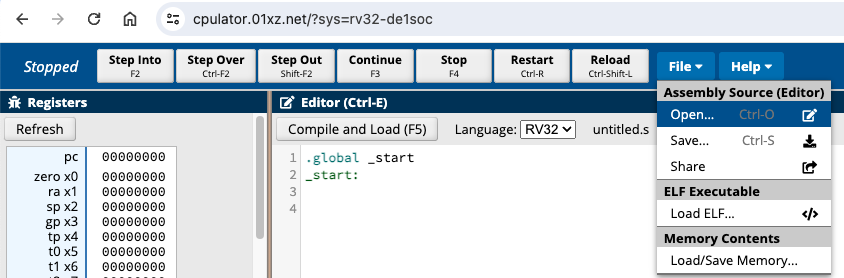
\includegraphics[width=\textwidth]{figures/file.png}}
	\end{center}
	\caption{The \texttt{File} menu in {\it CPUlator}.}
\label{fig:file}
\end{figure}

\begin{figure}[H]
	\begin{center}
    \setlength{\fboxsep}{0pt}
	\fbox{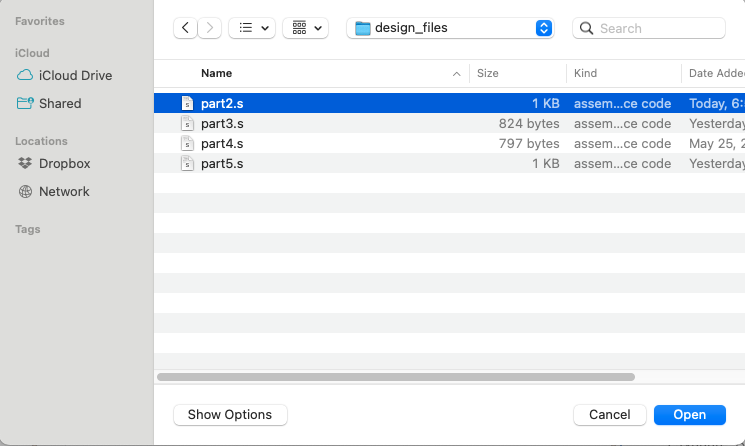
\includegraphics[scale=.5]{figures/open.png}}
	\end{center}
	\caption{Selecting the {\it part2.s} file.}
\label{fig:open}
\end{figure}

\begin{figure}[H]
	\begin{center}
    \setlength{\fboxsep}{0pt}
	\fbox{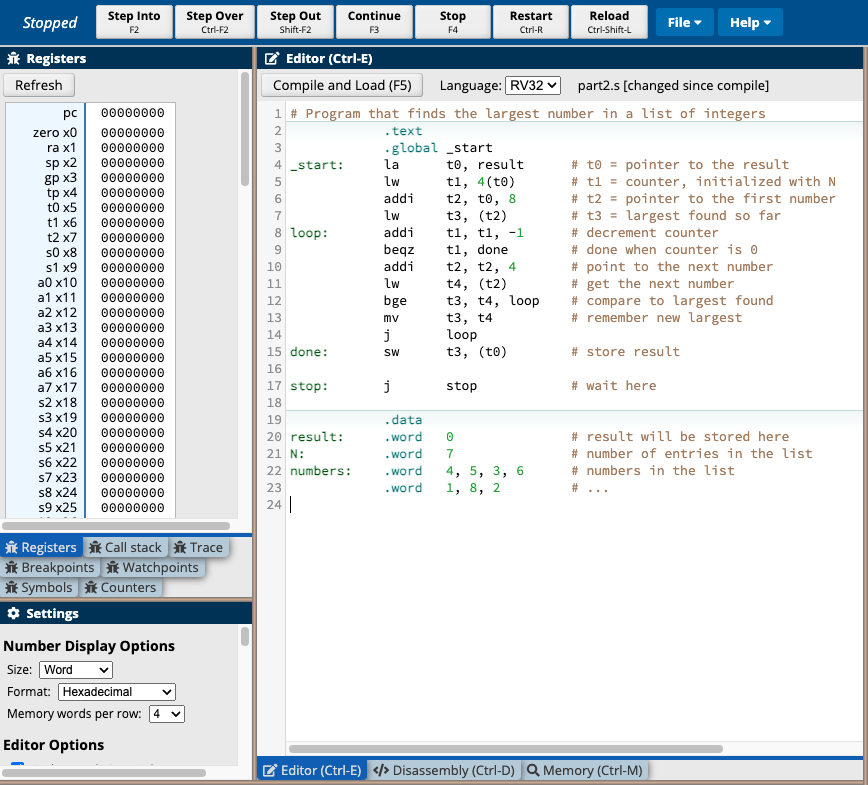
\includegraphics[scale=.5]{figures/editor.png}}
	\end{center}
	\caption{The assembly-language program in the {\it CPUlator} \texttt{Editor} pane.}
\label{fig:editor}
\end{figure}

~\\
\item As indicated in Figure~\ref{fig:compile}, click on the \fbox{\texttt{Compile and Load}}
command to {\it assemble} your program and {\it load} it into the {\it memory} that is
part of the computer system being simulated within the {\it CPUlator} tool. 
You should see the message displayed in Figure~\ref{fig:success}, in the \texttt{Messages} pane, 
which reports a successful compilation result.
If not, then you may have inadvertently introduced an error in the program code; fix any
such errors and recompile. 

Once the compilation is successful, the 
{\it CPUlator} window automatically displays the \texttt{Disassembly}
pane, shown in Figure~\ref{fig:end}. This pane lets you see the machine code for 
the program and gives the address in the {\it memory} of each machine-code word.
The \texttt{Disassembly} pane shows each instruction in the program twice: once using the 
original source code and a second time using the actual instruction found by {\it disassembling} 
the machine code. This is done because the {\it implementation} of an instruction 
may differ, in some cases, from the {\it specification} of that instruction in the source code 
(examples where such differences happen will be shown in class). Note: you can change the
way that code is displayed in the CPUlator by using its \texttt{Settings} menu, which is on
the left hand side of the CPUlator window (for example, changing \texttt{Disassembly Options} 
from {\it Some} to {\it None} will ensure that each instruction is displayed only once).
~\\
~\\

\begin{figure}[h]
	\begin{center}
    \setlength{\fboxsep}{0pt}
	\fbox{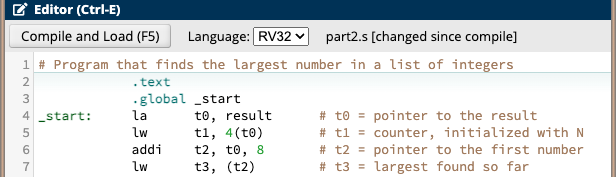
\includegraphics[scale=.5]{figures/compile.png}}
	\end{center}
	\caption{Compiling and loading the program.}
\label{fig:compile}
\end{figure}

\begin{figure}[h]
	\begin{center}
    \setlength{\fboxsep}{0pt}
	\fbox{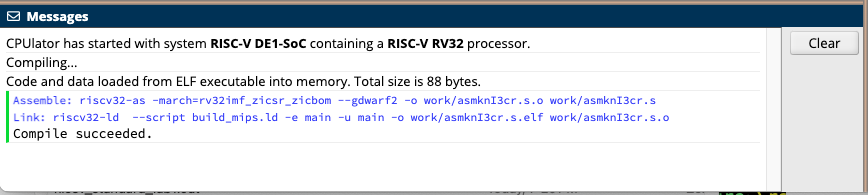
\includegraphics[scale=.5]{figures/success.png}}
	\end{center}
	\caption{The \texttt{Messages} pane.}
\label{fig:success}
\end{figure}

\item Select the \texttt{Continue} command near the top of the {\it CPUlator} window. This
command ``executes'' the program on the Nios~V processor that is part of the computer system 
being simulated within the {\it CPUlator} tool. 
As illustrated in Figure~\ref{fig:end}, the program runs to the line of code labeled
\texttt{stop}, at memory address \texttt{0x30}, where it remains in an endless loop.
Select the \texttt{Stop} command to halt the program's
execution.  Note that the largest number found in the sample list is 8 as indicated
by the contents of register \texttt{t3}. This result is also stored in memory at the label
{\it result}.  

\begin{figure}[H]
	\begin{center}
    \setlength{\fboxsep}{0pt}
	\fbox{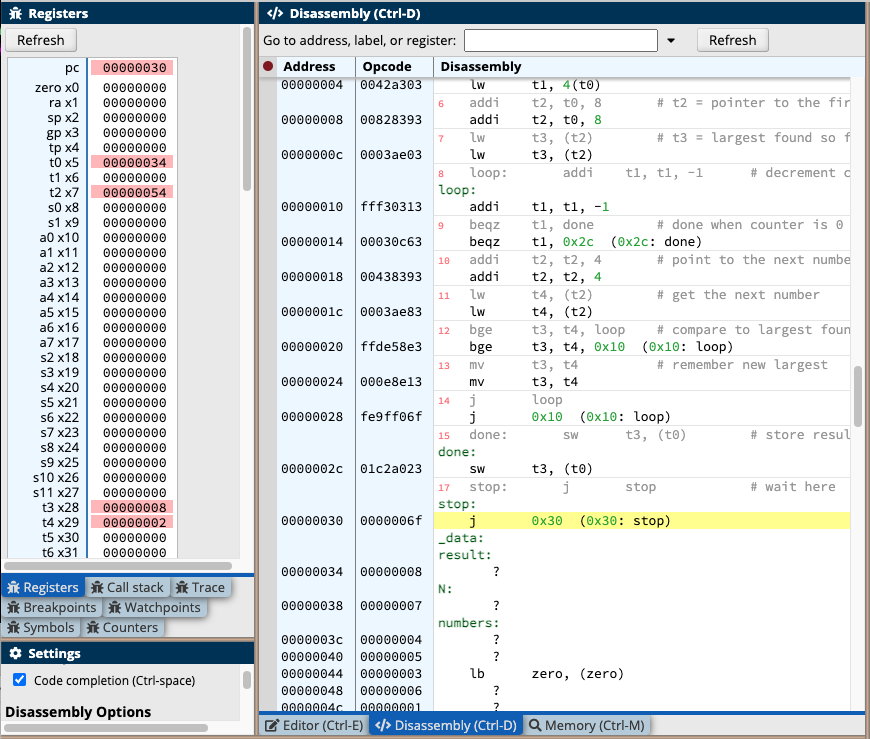
\includegraphics[scale=0.5]{figures/end.png}}
	\end{center}
	\caption{The result of executing the program.}
\label{fig:end}
\end{figure} 

~\\
~\\
The address of the label {\it result} is \texttt{0x00000034}, which can be seen
near the bottom of Figure~\ref{fig:end}. Also, you may notice that the
\texttt{Disassembly} pane attempts to figure out the machine code at this location,
assuming that it represents a processor instruction; it does not, and so the resulting
instruction displayed (\texttt{?}) is not meaningful. 

Use the {\it CPUlator's} \texttt{Memory} pane, as illustrated in Figure~\ref{fig:memory},
to verify that the resulting value 8 is stored in the correct location.

\begin{figure}[H]
	\begin{center}
    \setlength{\fboxsep}{0pt}
	\fbox{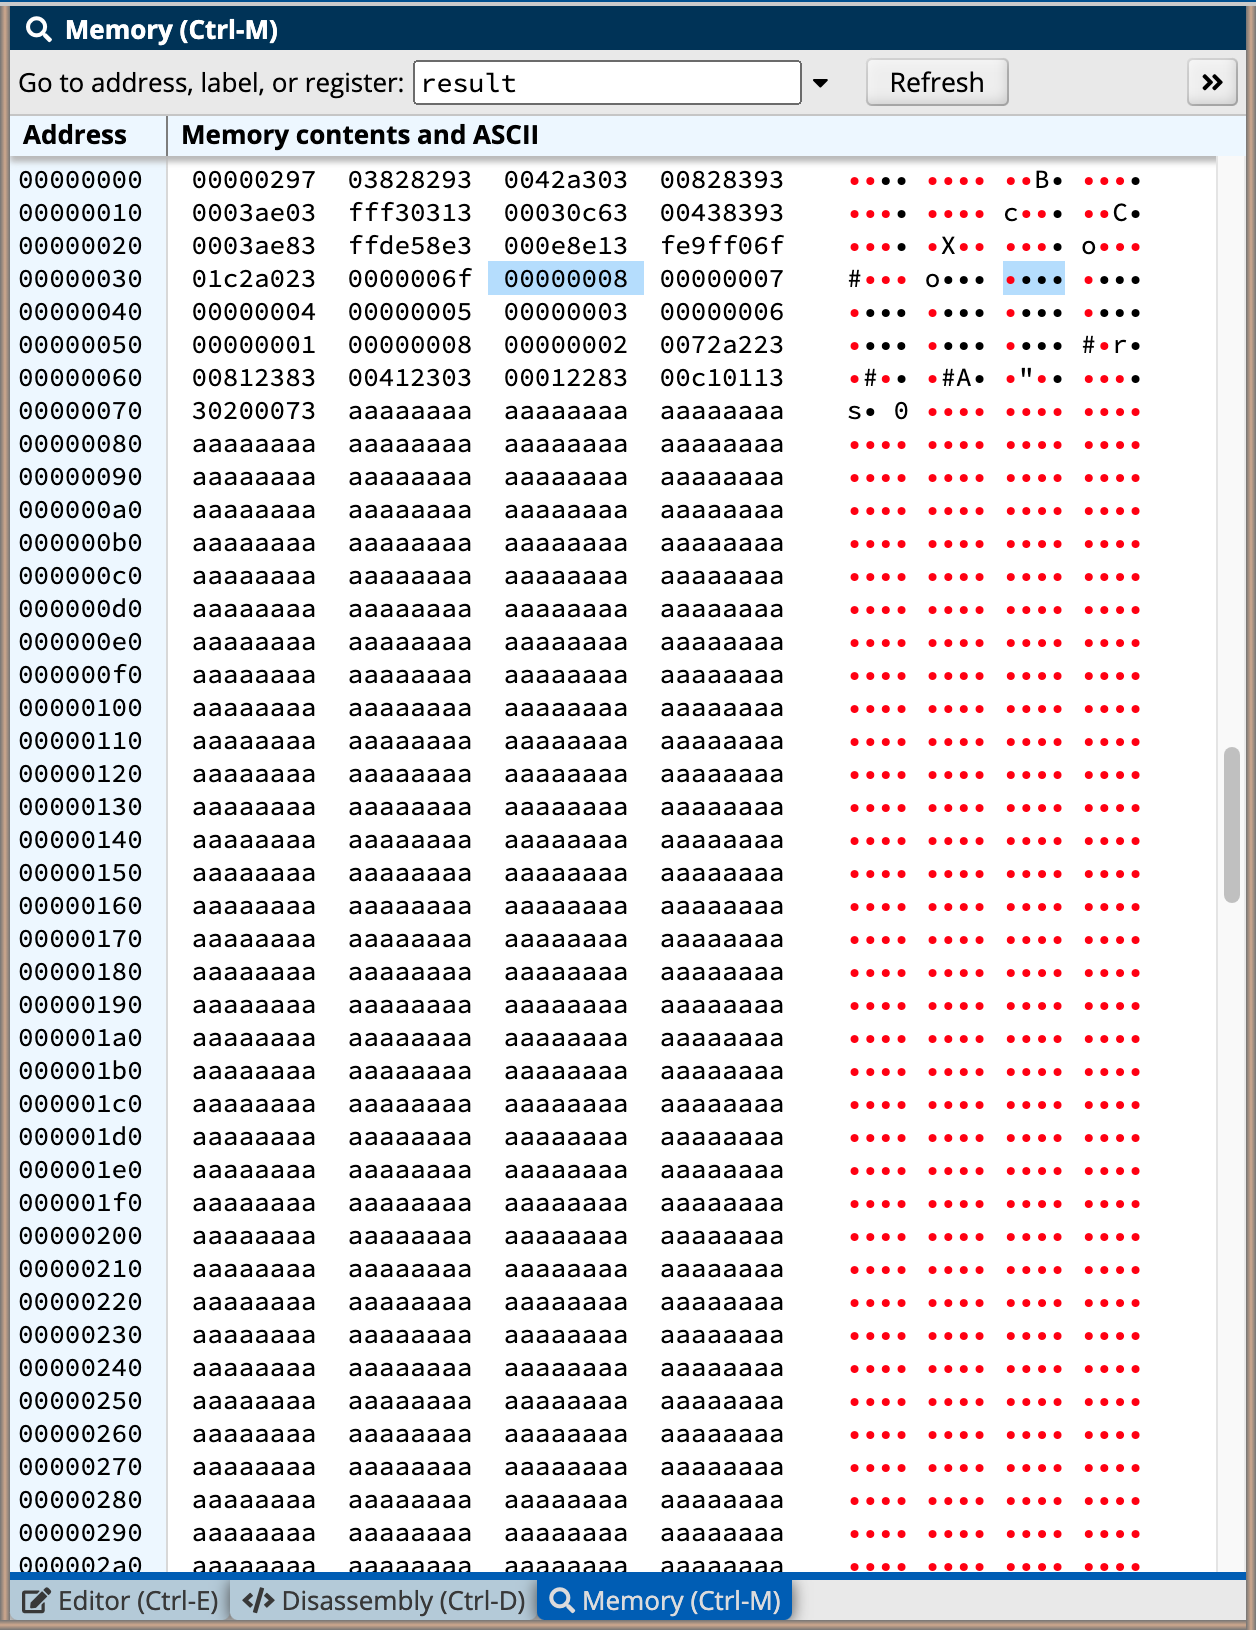
\includegraphics[scale=0.5]{figures/CPUlator_memory.png}}
	\end{center}
	\caption{The \texttt{Memory} pane.}
\label{fig:memory}
\end{figure} 

\item You can return control of the program to the start by clicking on the \texttt{Restart}
command in {\it CPUlator}.
Do this and then {\it single-step} through the program by (repeatedly) selecting the
\texttt{Step Into} command while observing the \texttt{Disassembly} pane.  
Observe how each instruction that is executed affects 
the contents of the Nios~V registers.

\item Double-click on the \texttt{pc} register in the {\it CPUlator} and then change the
value of the program counter to 0.  This action has the same effect as
selecting the \texttt{Restart} command. 

\item Now set a breakpoint at address \texttt{0x00000028} by clicking on the gray bar to
the left of this address, as illustrated in Figure~\ref{fig:bp}. Select the \texttt{Continue}
command to run the program again and observe the contents of register \texttt{t3} when 
the instruction at the breakpoint, which is \texttt{j loop}, is reached. Use 
\texttt{Continue} to repeatedly run the program, which will stop at the breakpoint in each
iteration of the loop, and monitor 
the contents of register \texttt{t3} as the program searches for 
the largest number in the list.

\begin{figure}[H]
	\begin{center}
    \setlength{\fboxsep}{0pt}
	\fbox{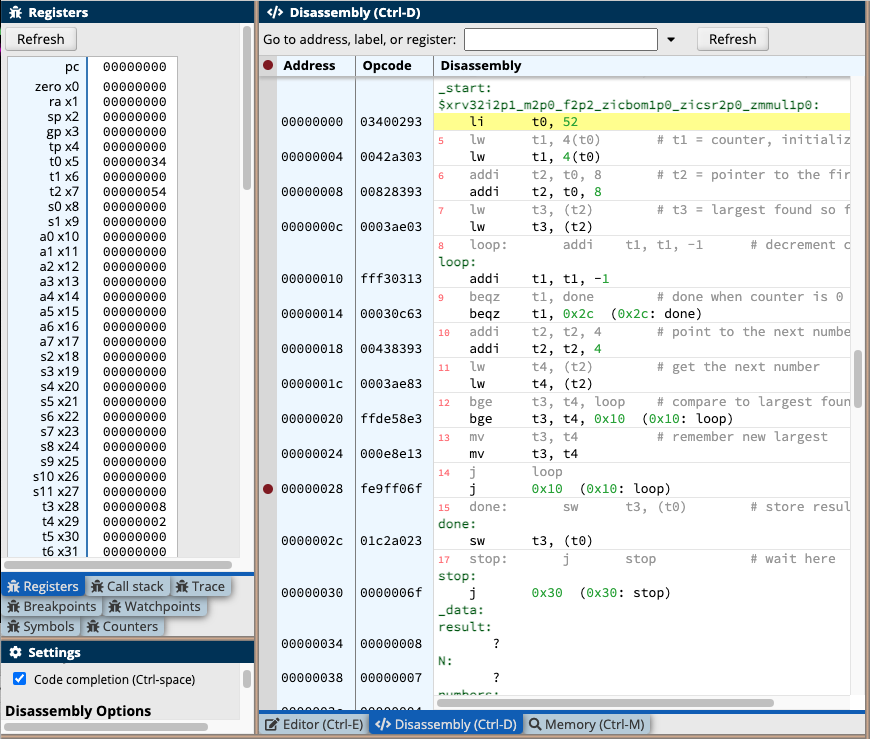
\includegraphics[scale=0.5]{figures/bp.png}}
	\end{center}
	\caption{Setting a breakpoint.}
\label{fig:bp}
\end{figure} 

\end{enumerate}

~\\
\section*{Part III}

Implement the task in Part II by modifying the program in Figure~\ref{fig:code} so that it
uses a subroutine. The subroutine, named {\it large}, has to find the largest number in a list.
The main program passes the number of entries and the address of the start of the
list as parameters to the subroutine via registers {\it a0} and {\it a1} respectively.
The subroutine returns the value of the largest number to the calling program
via register {\it a0}. A suitable main program is given in Figure~\ref{fig:main}.
~\\

\noindent
Use the {\it CPUlator} tool to assemble, load, execute, and debug (as needed!) your program. 

\begin{figure}[h]
\begin{center}
\lstinputlisting[style=defaultNiosVStyle]{../design_files/part3.s}
\end{center}
\caption{Main program for Part III.}
\label{fig:main}
\end{figure}

\newpage
\section*{Part IV}

The program shown in Figure~\ref{fig:reverse} reads a string of characters (bytes) from
the memory and reversing the string in-place. The string is created in the memory by using
the \texttt{.asciz} assembler directive, which generates the ASCII code for each character
in the string and places these bytes into the memory starting at the address of 
the {\it string} label.

~\\
\noindent
The program works by first setting a pointer
to the beginning of the string, and then identifying, using the loop labeled 
\texttt{zloop}, the location in memory of the last character in the string. Next, in the 
loop labeled \texttt{reverse}, the program swaps the two characters 
at the ends the string, and then the ones next to those on each end,
and so on, working toward the middle of the string until done. 

~\\
\noindent
~\\
\noindent
Perform the following:

\setlength{\fboxsep}{1pt}
\begin{enumerate}
\item Create an assembly-language source-code file for the program in
Figure~\ref{fig:reverse}, and name the file {\it part4.s} (this file is included in 
the {\it design files} for this lab exercise). Then, enter this code into 
the {\it CPUlator} tool.
\item
Make use of the {\it CPUlator} features, such as single-stepping, setting breakpoints, 
examining registers and the contents of memory, and so on, to ensure that
you thoroughly understand how the code in Figure~\ref{fig:reverse} works.
Make sure that you examine the {\it string} in the \texttt{Memory} tab of the {\it CPUlator}, 
both before and after it has been reversed. Note that the ASCII characters of the string
are displayed on the right-hand side of the \texttt{Memory} tab.
\end{enumerate}

\begin{figure}[H]
\begin{center}
\lstinputlisting[style=defaultNiosVStyle]{../design_files/part4.s}
\end{center}
\caption{A program that reverses a text string.}
\label{fig:reverse}
\end{figure}

\section*{Part V}

Implement the task in Part IV by modifying the program in Figure~\ref{fig:reverse} so that it
uses two subroutines. One subroutine, named {\it slen}, has to find the number of
characters in the string that is to be reversed (not counting the zero at the
end). The main program passes to {\it slen} a pointer to the first character in the string,
in register {\it a0}.  The other subroutine, named {\it srev}, performs the string reversal. 
Its parameters are a pointer to the first character in the string, in register {\it a0}, and 
a pointer to the last character in the string, in register {\it a1}. 
~\\

\noindent
A suitable main program is given in Figure~\ref{fig:main2}. It reserves two strings by
using the {\it slen} and {\it srev} subroutines. 
Use the {\it CPUlator} to assemble, load, execute, and debug (as needed!) your program. 
Note that the \texttt{.align} assembler directive used in Figure~\ref{fig:main2}
causes each string to be placed in the memory at a 16-byte boundary; this alignment starts
each string on a separate line of the \texttt{Memory} tab in the {\it CPUlator}, making
it easier for you to visually examine the strings.

\begin{figure}[H]
\begin{center}
\lstinputlisting[style=defaultNiosVStyle]{../design_files/part5.s}
\end{center}
\caption{Main program for Part V.}
\label{fig:main2}
\end{figure}

\newpage
\subsection*{Part VI: Introduction to the Monitor Program}

\noindent
This part of the exercise introduces the {\it Monitor Program} application software, which 
allows you to develop and debug Nios~V code that is being executed on a
{\it real} DE1-SoC board. As stated earlier in this exercise, you cannot use the 
{\it CPUlator} to control a real hardware board, because the {\it CPUlator} only 
{\it simulates} the features of the DE1-SoC Computer and does not use the actual hardware.

~\\
\noindent
To use the Monitor Program software, your computer must be connected by a USB cable to a 
DE1-SoC board (the cable has to be plugged into the {\it USB Blaster} port on the board).
In a similar manner as described earlier in this exercise (when using the {\it CPUlator}), you 
will develop software code that runs on the DE1-SoC Computer, 
which includes Nios~V, memory, and various I/O devices.
However, in this case you are not using a {\it simulation} of the DE1-SoC Computer. Instead, 
the {\it DE1-SoC Computer} is implemented as a circuit which is downloaded by the Monitor
Program application into the FPGA device on the DE1-SoC board. You use the Monitor Program to 
control the Nios~V processor on the board.

~\\
\noindent
The remaining parts of this exercise require the use of a DE1-SoC board. The Monitor
Program cannot be used at all without a hardware board attached to your computer.

~\\
\noindent
The first step in using the Monitor Program is to set up a Nios~V software development
project.  Perform the following:
\begin{enumerate}
\item Make sure that the power is turned on for the DE1-SoC board.
\item Open the {\it Monitor Program} software, which leads to the window in Figure~\ref{fig:MP1}.

\noindent
To develop Nios~V software code using the Monitor Program it is necessary to create a new project.
Select {\sf File $>$ New Project} to reach the window in Figure~\ref{fig:MP2}.
Give the project a name and indicate the folder for the project; 
we have chosen the project name {\it part1} in the folder {\it Exercise1$\backslash$Part1},
as indicated in the figure. Use the drop-down menu shown in Figure~\ref{fig:MP2} to set
the target architecture to Nios~V.
Click {\sf Next}, to get the window in Figure~\ref{fig:MP3}.

\item Now, you can select your own custom computer system (if you have one) or a 
pre-designed (by Altera) system. As shown in Figure~\ref{fig:MP3} select the 
{\it DE1-SoC Computer}. Once you have selected the computer system the display in the window 
will now show where files that implement the chosen system are located. 
Click {\sf Next}.

\begin{figure}[H]
	\begin{center}
	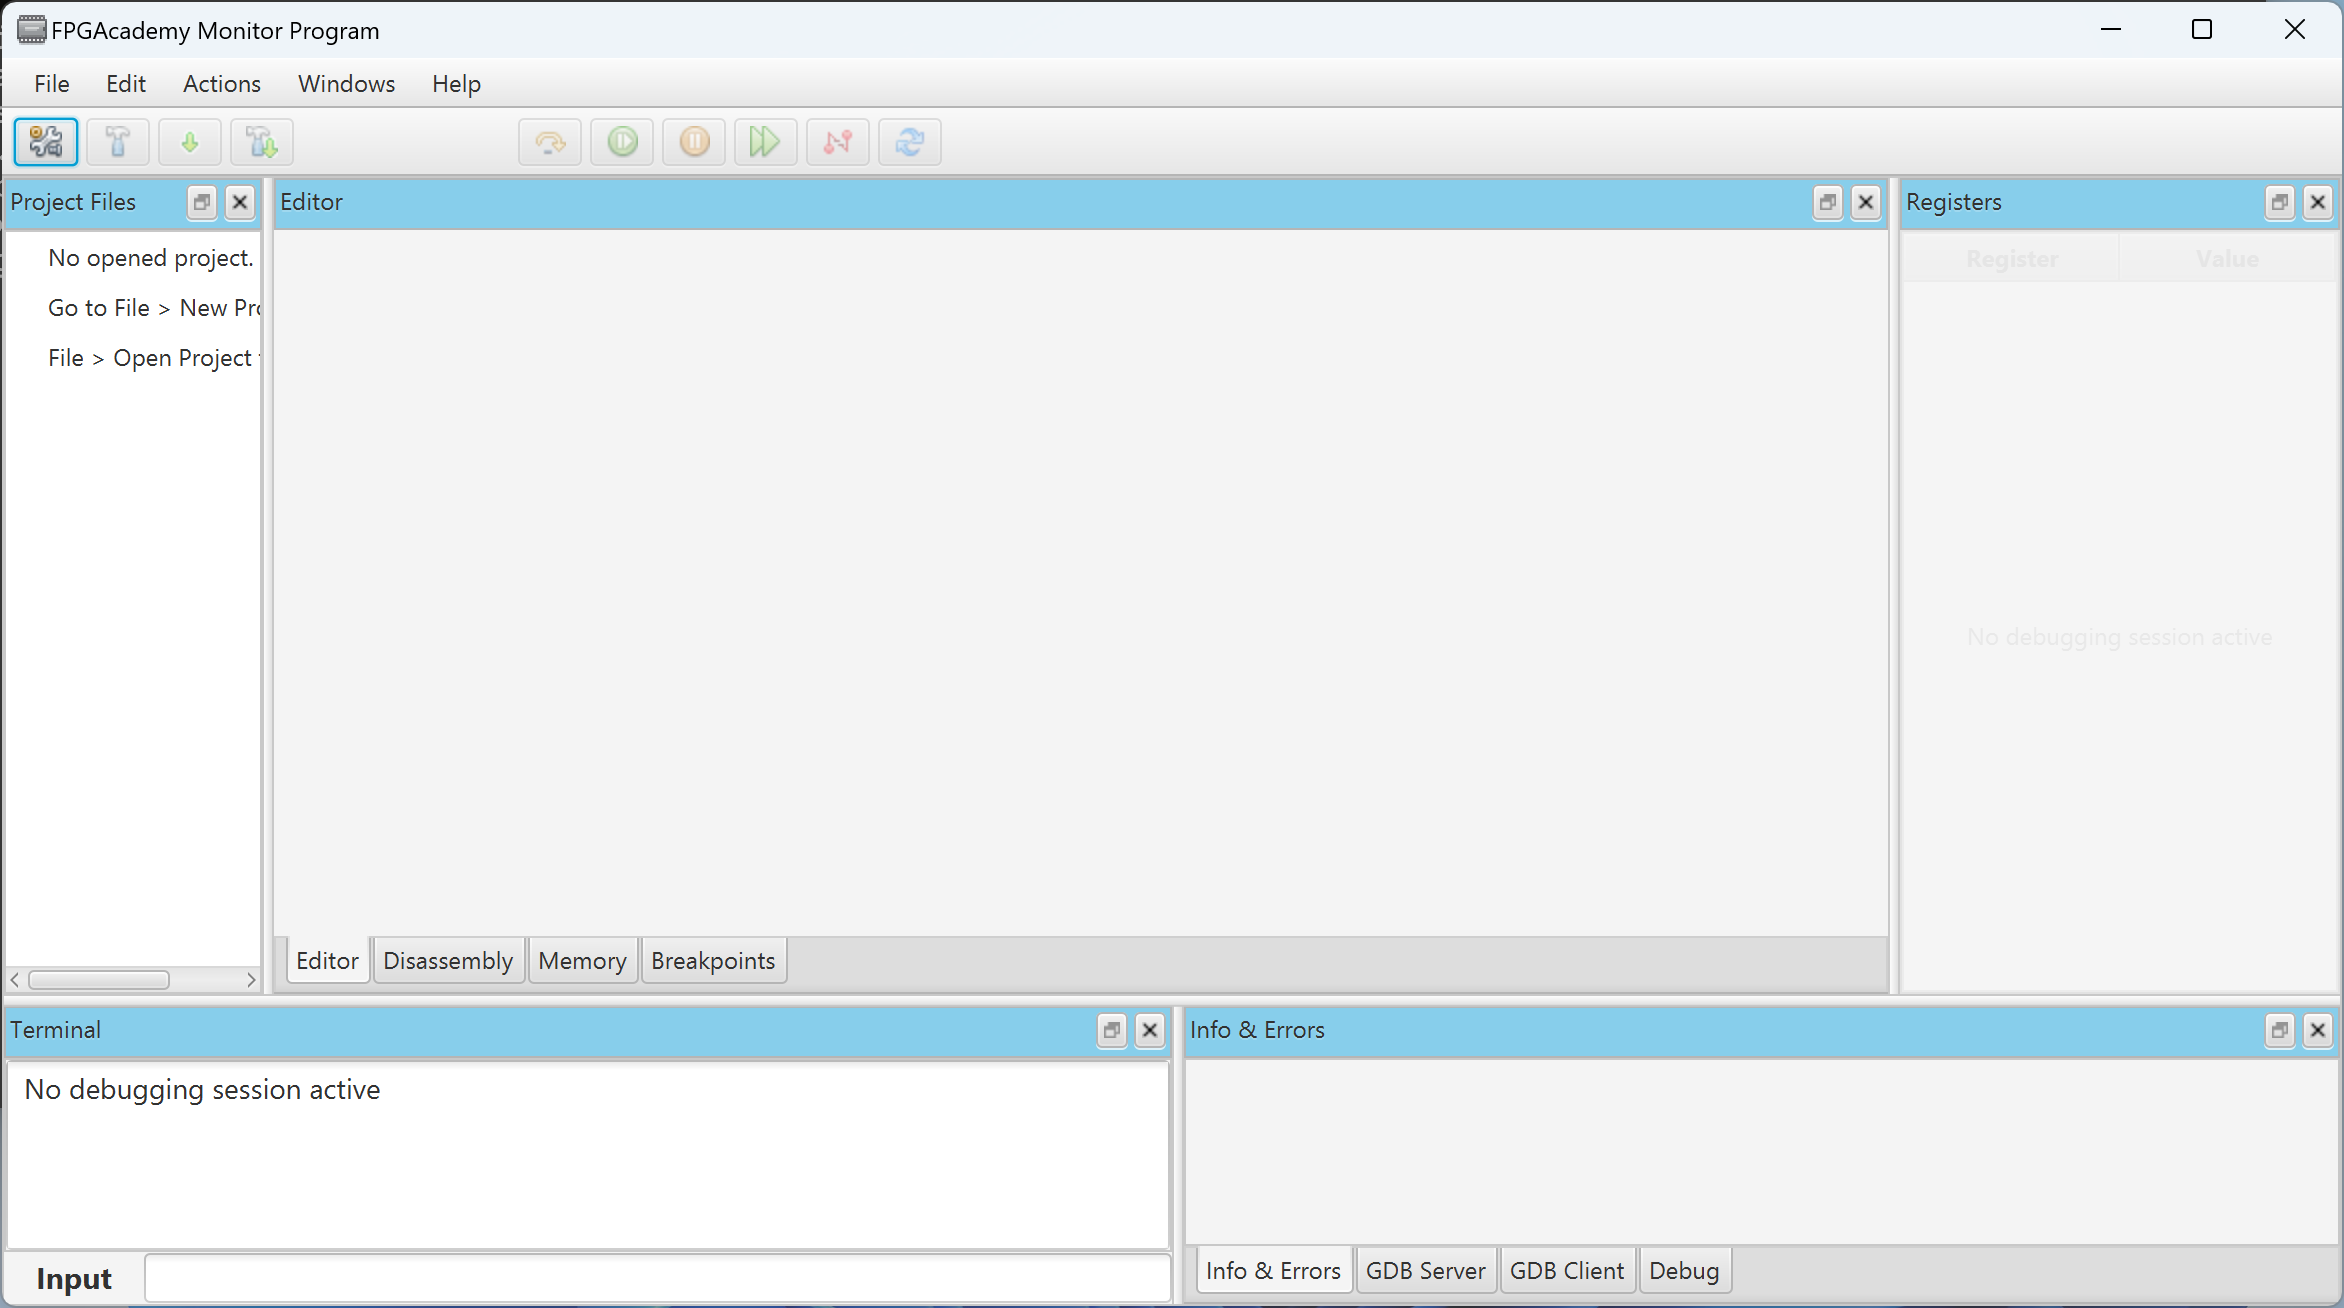
\includegraphics[scale=.33]{figures/Snap1.png}
	\end{center}
	\caption{The {\it Monitor Program} window.}
\label{fig:MP1}
\end{figure}

\begin{figure}[H]
	\begin{center}
	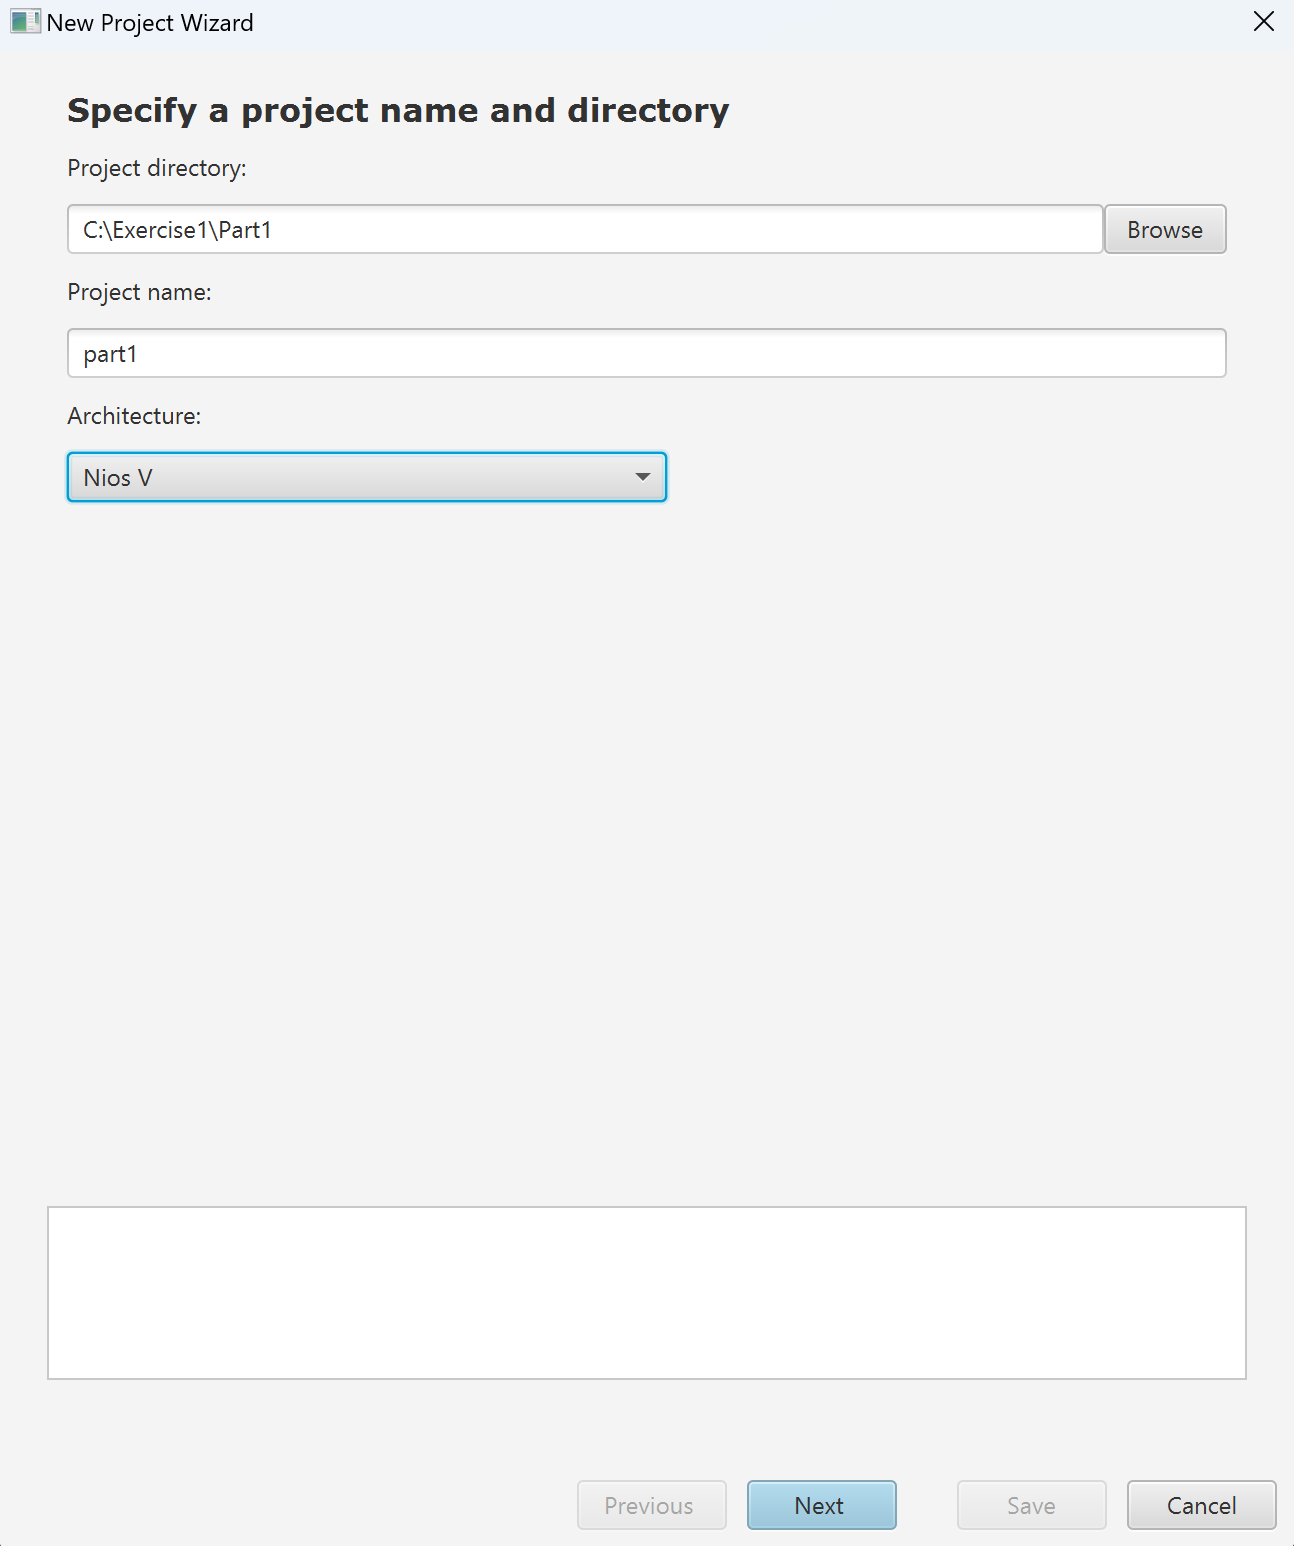
\includegraphics[scale=0.33]{figures/Snap2.png}
	\end{center}
	\caption{Specify the folder and the name of the project.}
\label{fig:MP2}
\end{figure}

\begin{figure}[H]
	\begin{center}
	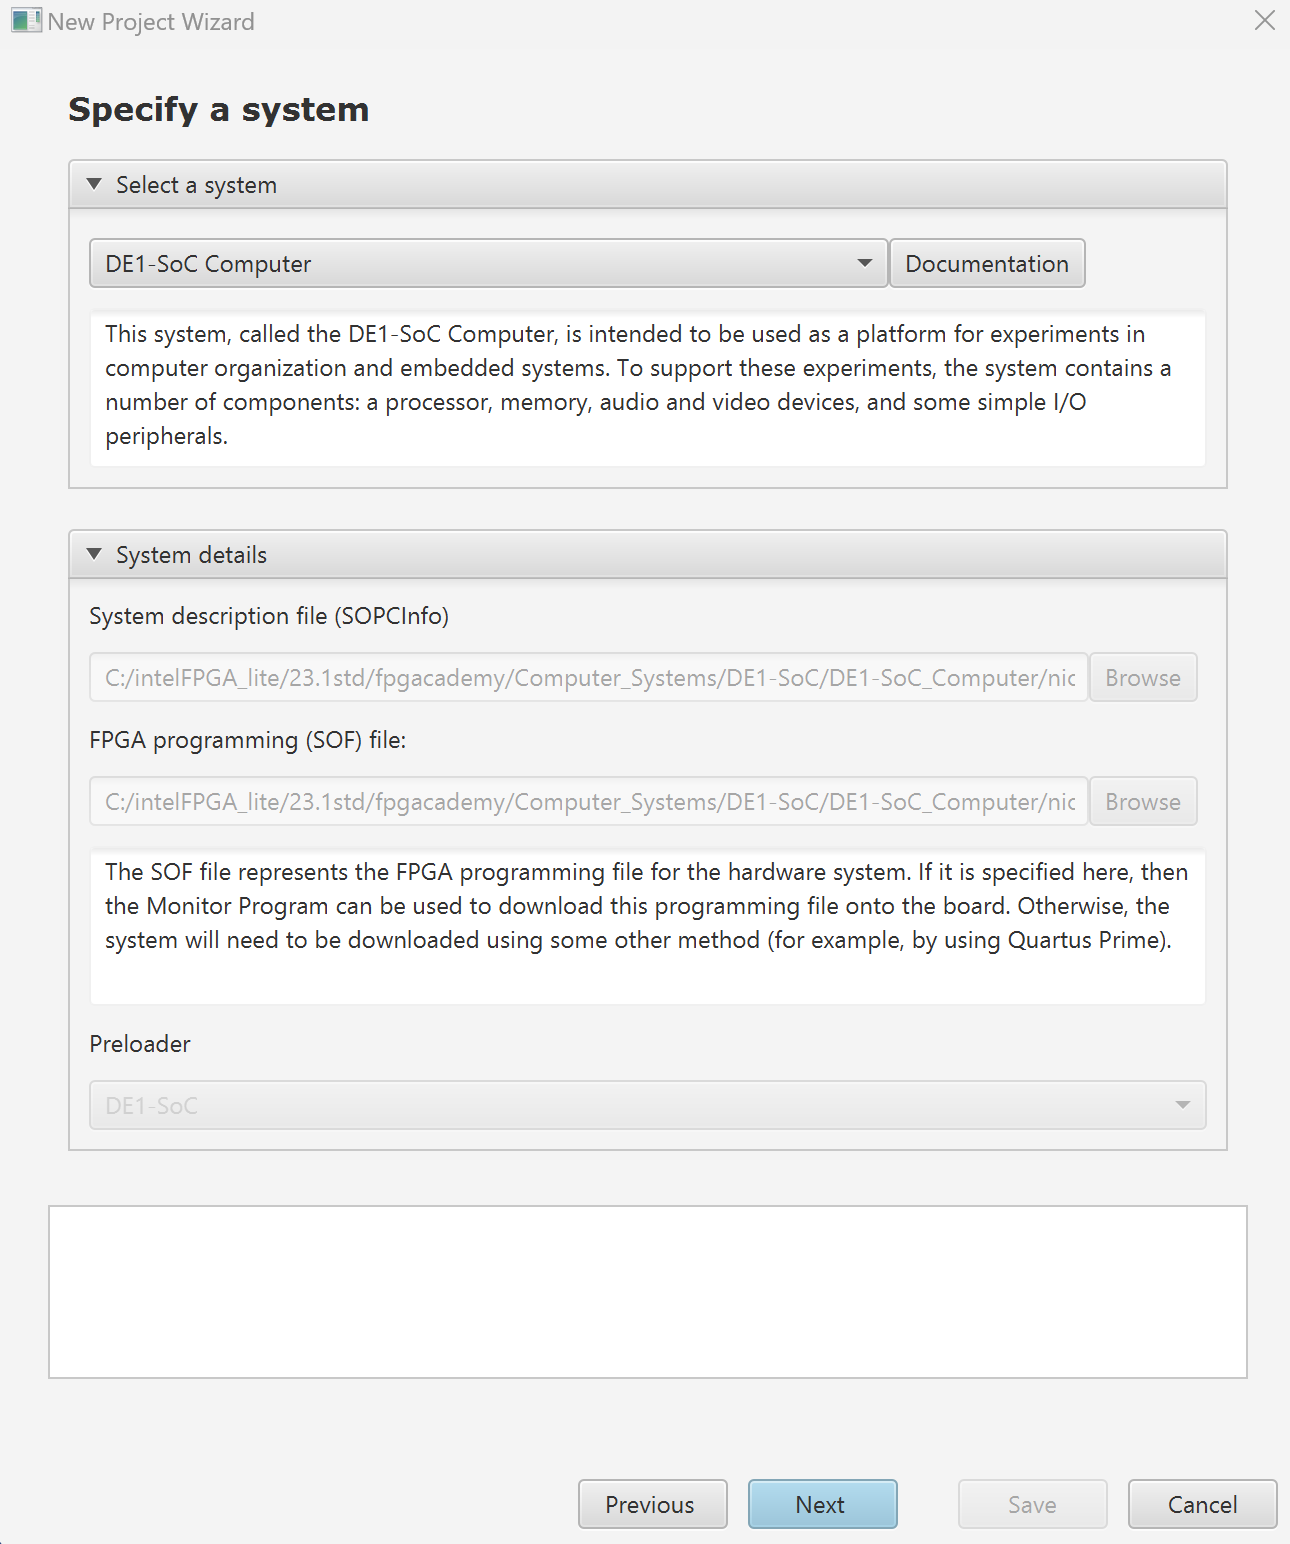
\includegraphics[scale=0.33]{figures/Snap3.png}
	\end{center}
	\caption{Specification of the system.}
\label{fig:MP3}
\end{figure}

\item In the window in Figure~\ref{fig:MP4} you can specify the type of application 
programs that you wish to run. They can be written in either assembly language
or the C programming language.  Specify that an assembly language program will be used. 
The {\it Monitor Program} package contains several sample programs.
Select the box {\sf Include a sample program with the project}.
Then, choose the {\sf Getting Started} program, as indicated in the figure, and 
click {\sf Next}.

\item The window in Figure~\ref{fig:MP5} is used to specify the source file(s) that contain the
application program(s).
Since we have selected the {\it Getting Started} program, the window indicates the source
code file for this program. This window also allows the user to specify the starting point in the
selected application program. The default symbol is {\it \_start}, which is used
in the selected sample program. Click {\sf Next}. 

\item The window in Figure~\ref{fig:MP6} indicates some system parameters.
Note that the figure indicates that the {\it DE-SoC [USB-1]} cable is selected to provide 
the connection between the DE-series board and the host computer.  This is the name assigned 
to the Altera USB Blaster connection between the computer and the board.  
If no \texttt{Host Connection} is shown, click on the \texttt{Refresh} button. 


\begin{figure}[H]
	\begin{center}
	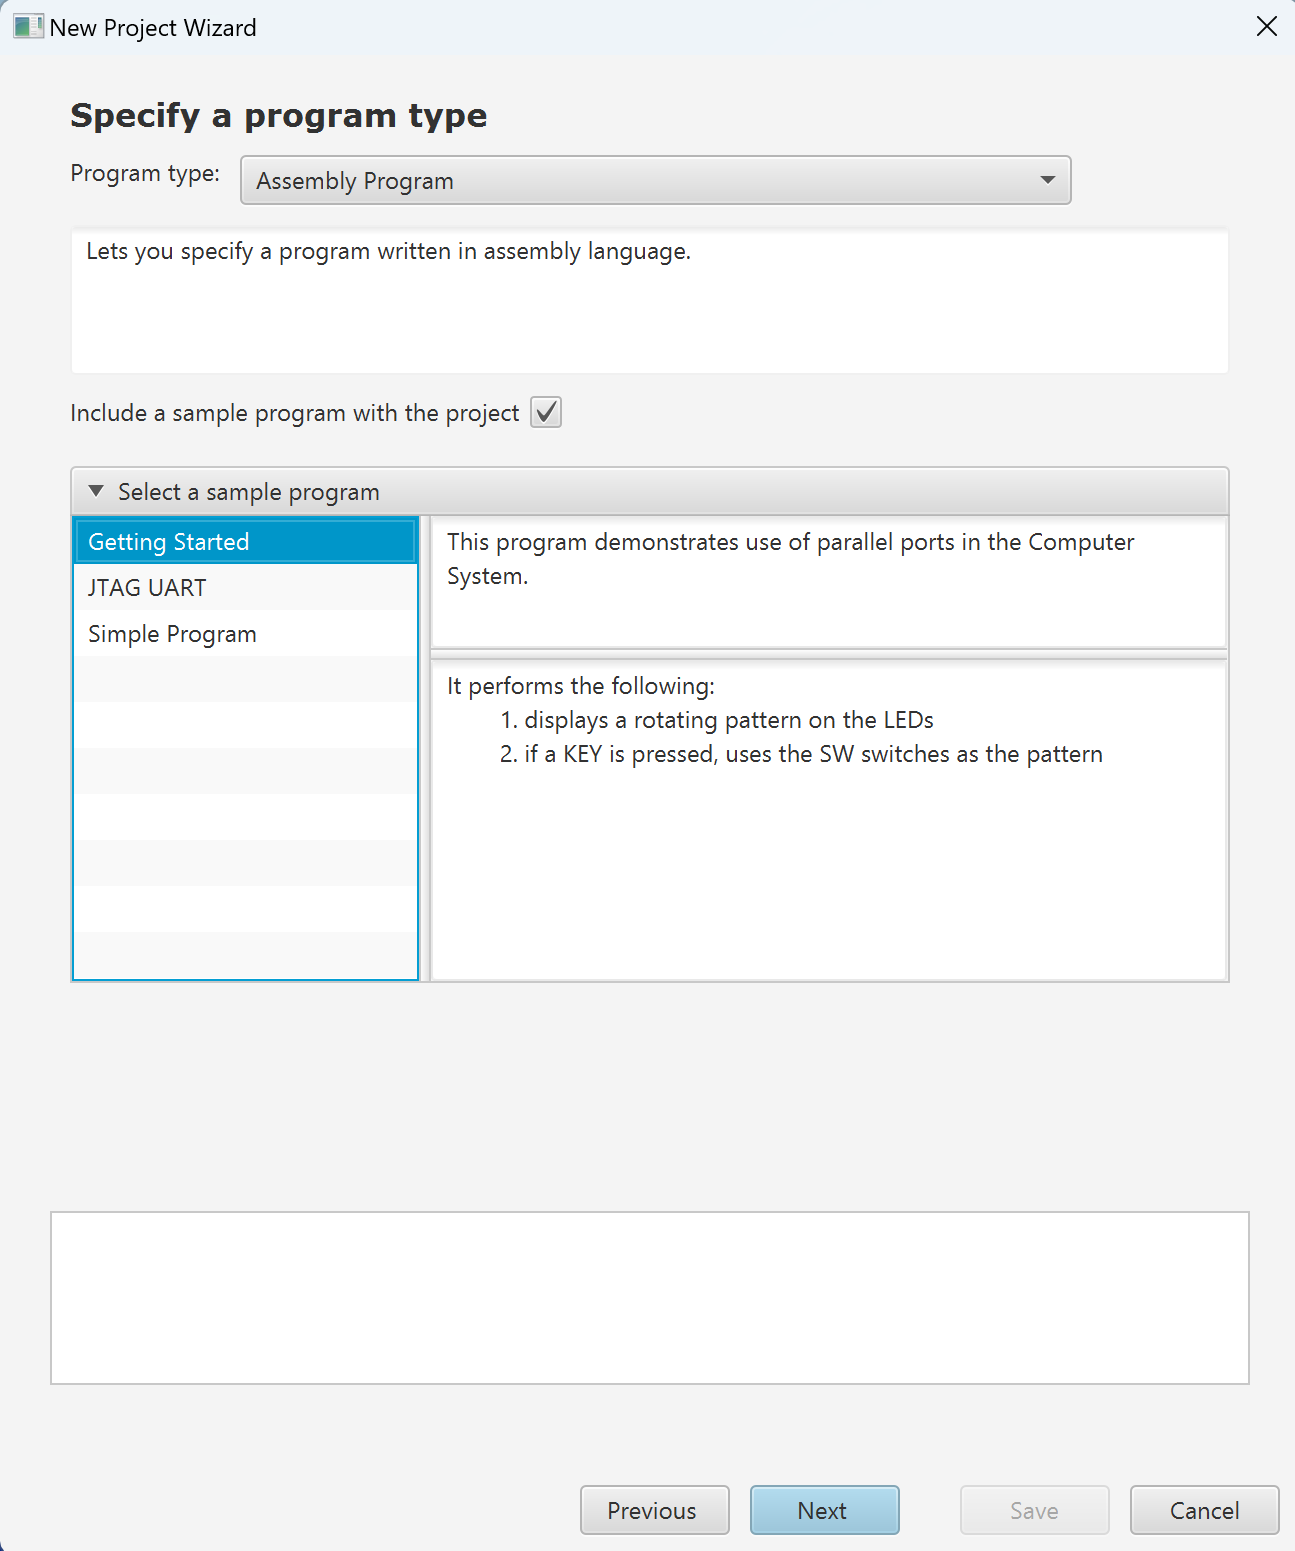
\includegraphics[scale=0.3]{figures/Snap4.png}
	\end{center}
	\caption{Selection of an application program.}
\label{fig:MP4}
\end{figure}

\begin{figure}[H]
	\begin{center}
	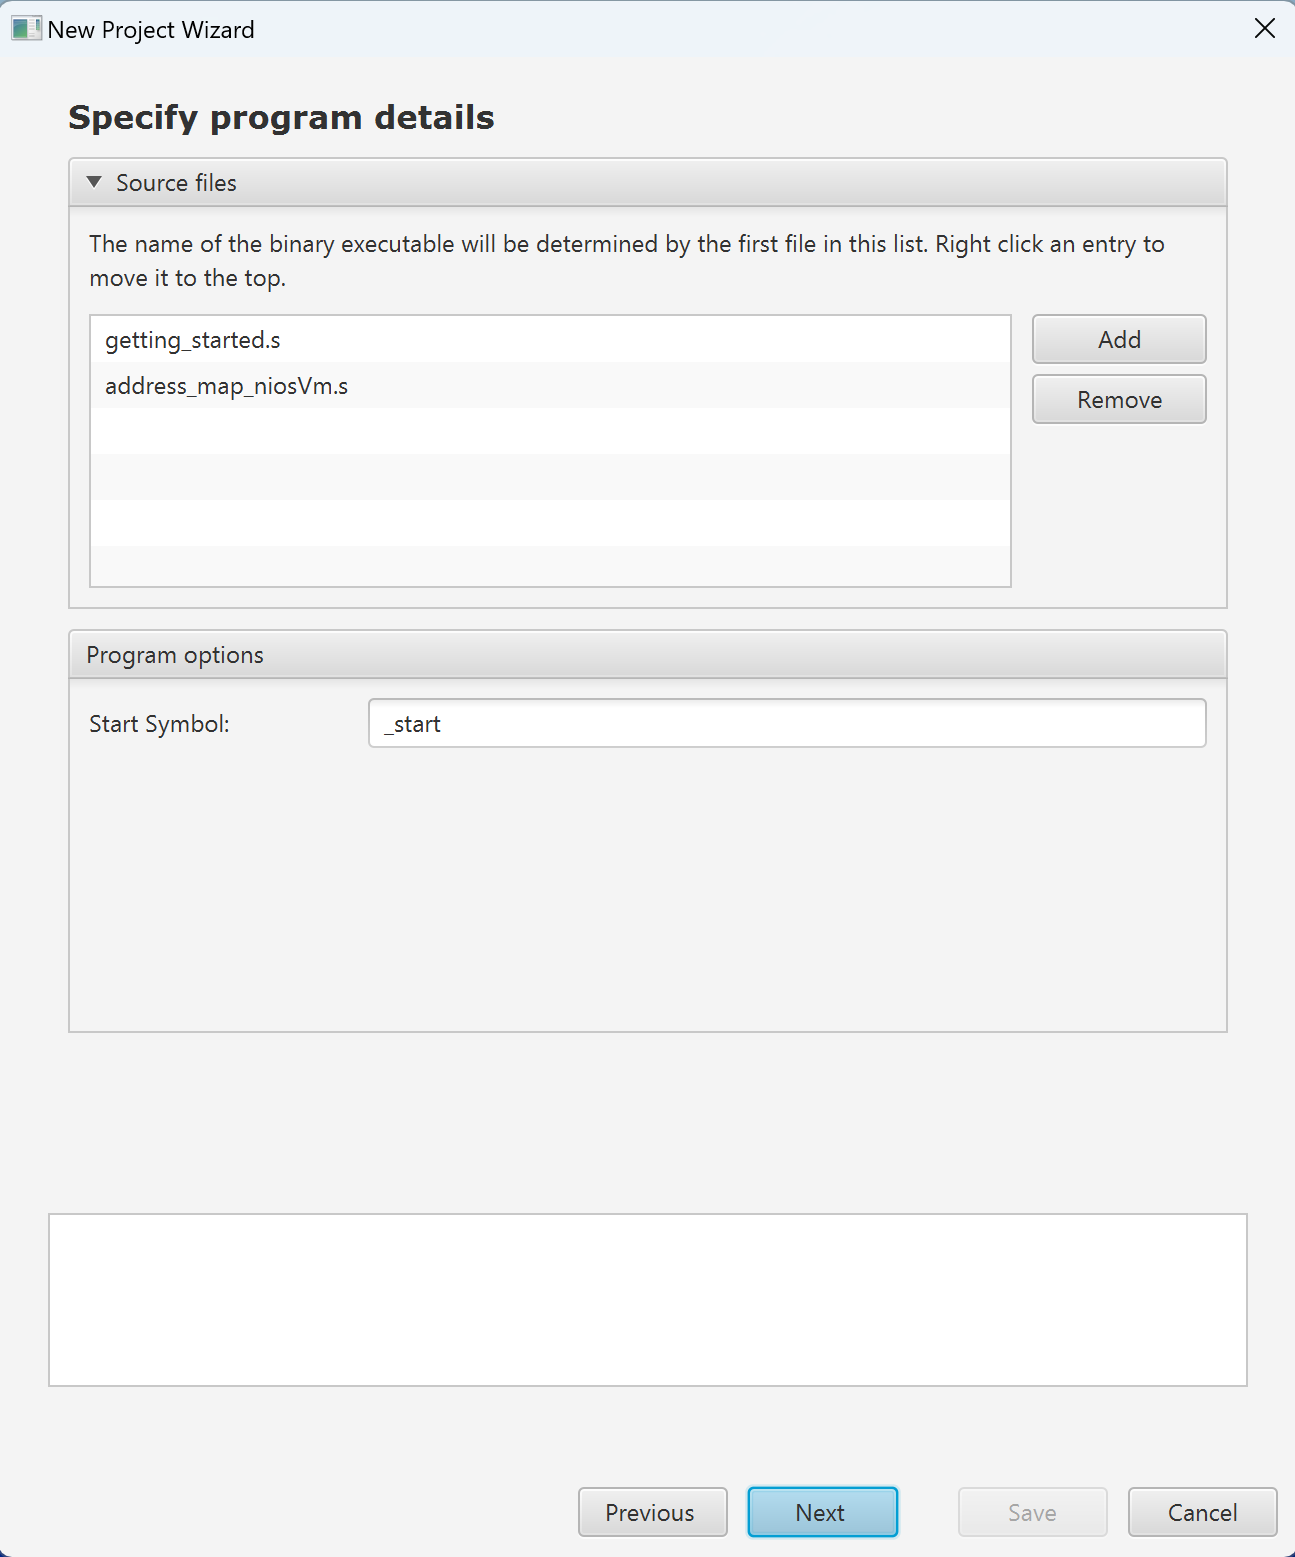
\includegraphics[scale=0.3]{figures/Snap5.png}
	\end{center}
	\caption{Source files used by the application program.}
\label{fig:MP5}
\end{figure}

\begin{figure}[H]
	\begin{center}
	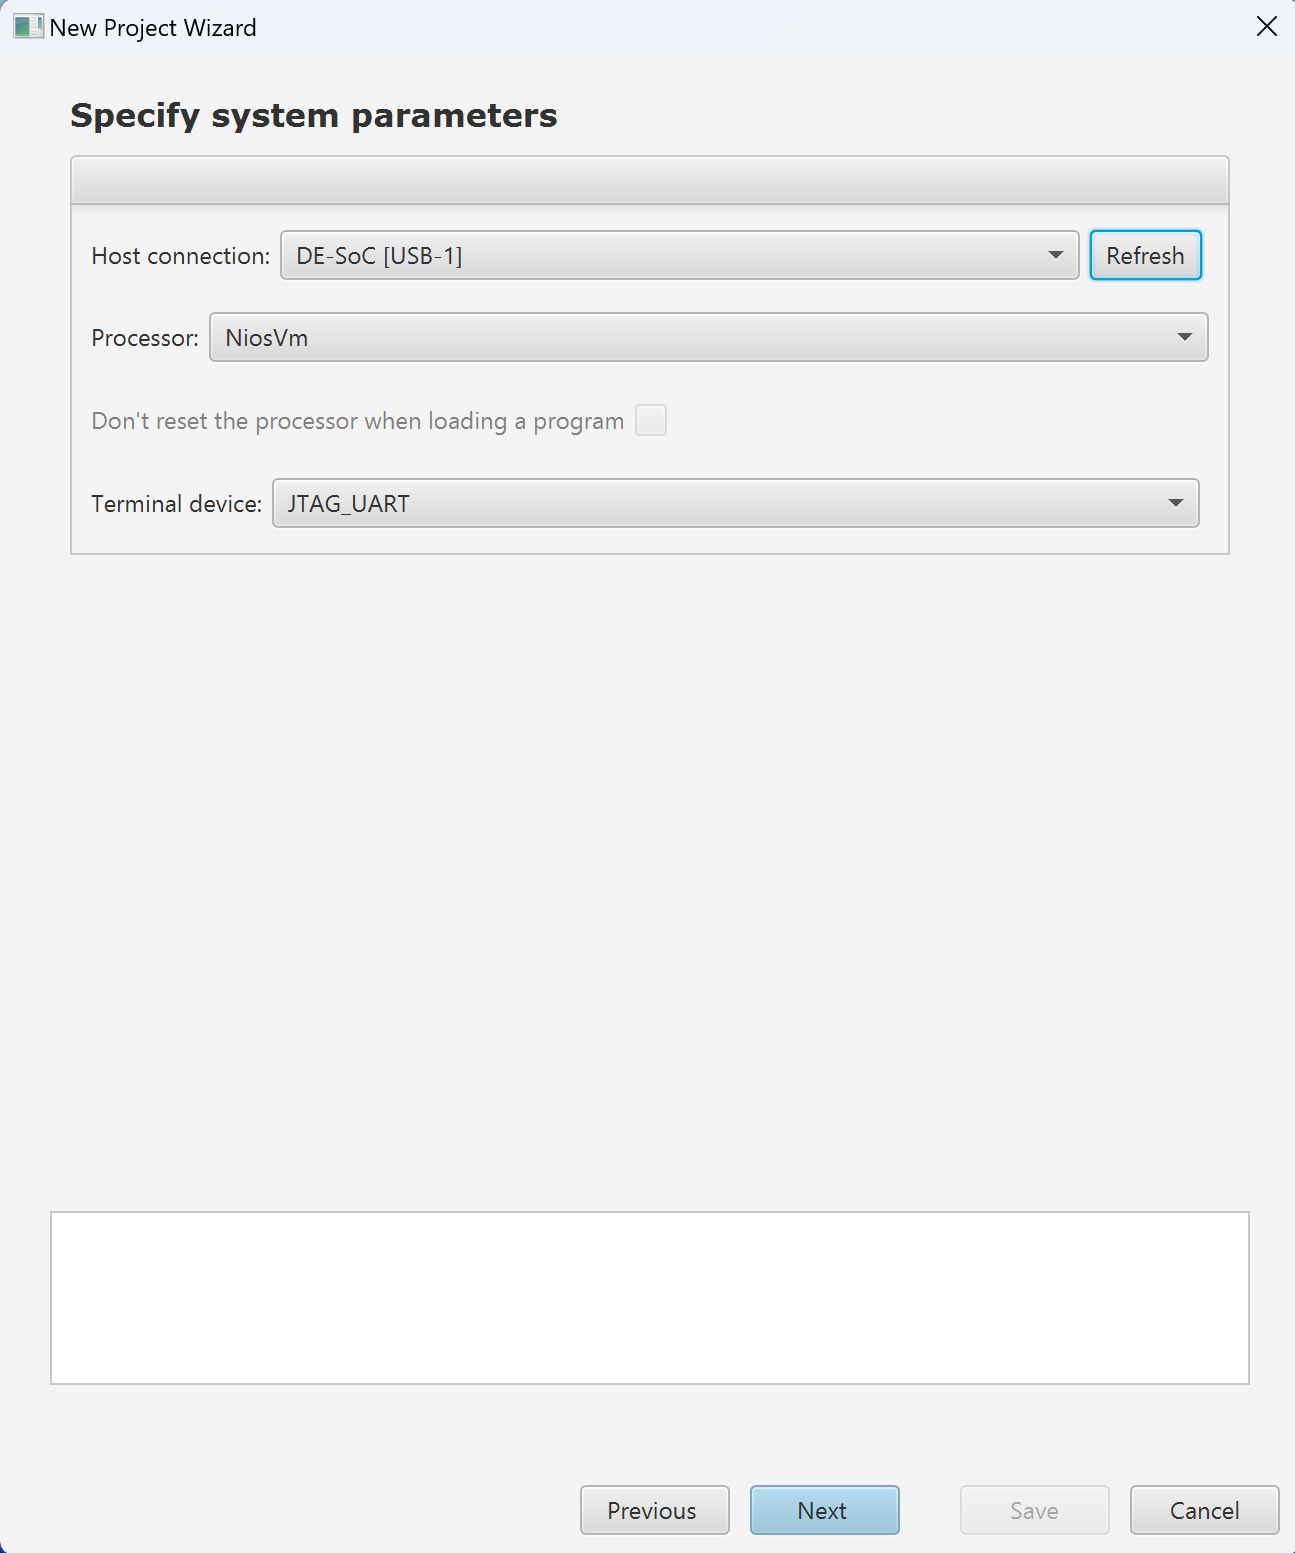
\includegraphics[scale=0.33]{figures/Snap6.png}
	\end{center}
	\caption{Specify the system parameters.}
\label{fig:MP6}
\end{figure}

\item The window in Figure~\ref{fig:MP7} displays the names of Assembly sections that will
		  be used for the program, and allows the user to select a target memory location
		  for each section. In this case only the .{\it text} section, which corresponds to
		  the program code (and data), will be used. As shown in the figure, the .{\it text}
		  section is targeted to the memory in the DE-series board that is mapped to start at
		  address 0. 
Click {\sf Save} to complete the specification of the new project.

\item After your project is saved, you can download the DE1-SoC Computer to your board.
Click on \texttt{Actions $>$ Download system}. Observe the messages in the 
\texttt{Info \& Errors} area in the Monitor Program screen
to see when the {\it Quartus Programmer}, which performs the download, is finished. 

\begin{figure}[H]
	\begin{center}
	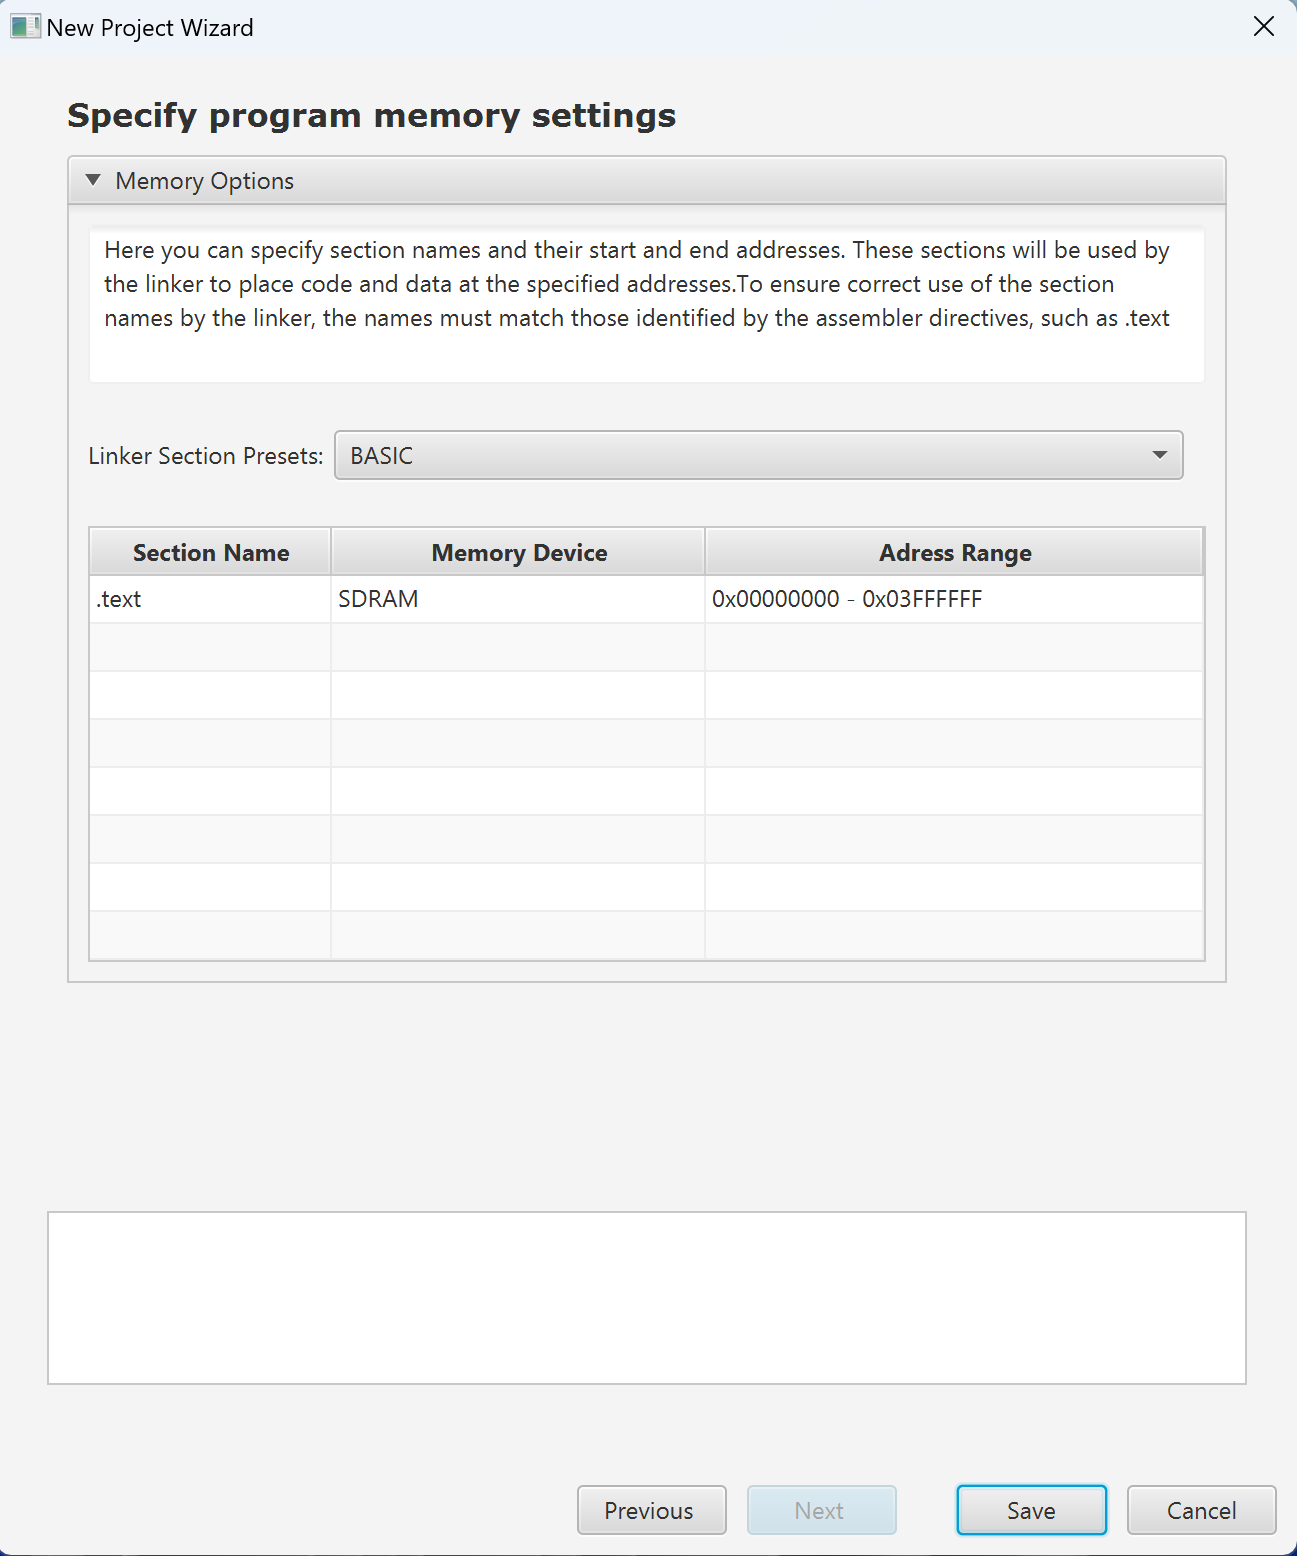
\includegraphics[scale=0.33]{figures/Snap7.png}
	\end{center}
	\caption{Specify the program memory settings.}
\label{fig:MP7}
\end{figure}

\item Having downloaded the computer system into the FPGA on your DE1-SoC board, 
we can now load and run the sample program.
In the main Monitor Program window, shown in Figure~\ref{fig:MP9}, 
select {\sf Actions $>$ Compile \& Load} 
to assemble the program and load it into the memory on the board.
Figure~\ref{fig:MP9} shows the Monitor Program window after the sample program has been loaded. 
\item Run the program by selecting {\sf Actions $>$ Continue} or
by clicking on the toolbar icon \hbox{
\includegraphics[scale=0.45]{figures/Cont.png}}, 
and observe the patterns displayed on the LEDs. 
\item Pause the execution of the sample program by clicking on the 
icon \hbox{
\includegraphics[scale=0.4]{figures/Pause.png}}, 
and disconnect from this session
by clicking on the icon \hbox{
\includegraphics[scale=0.45]{figures/Disconn.png}}, 

\begin{figure}[H]
	\begin{center}
	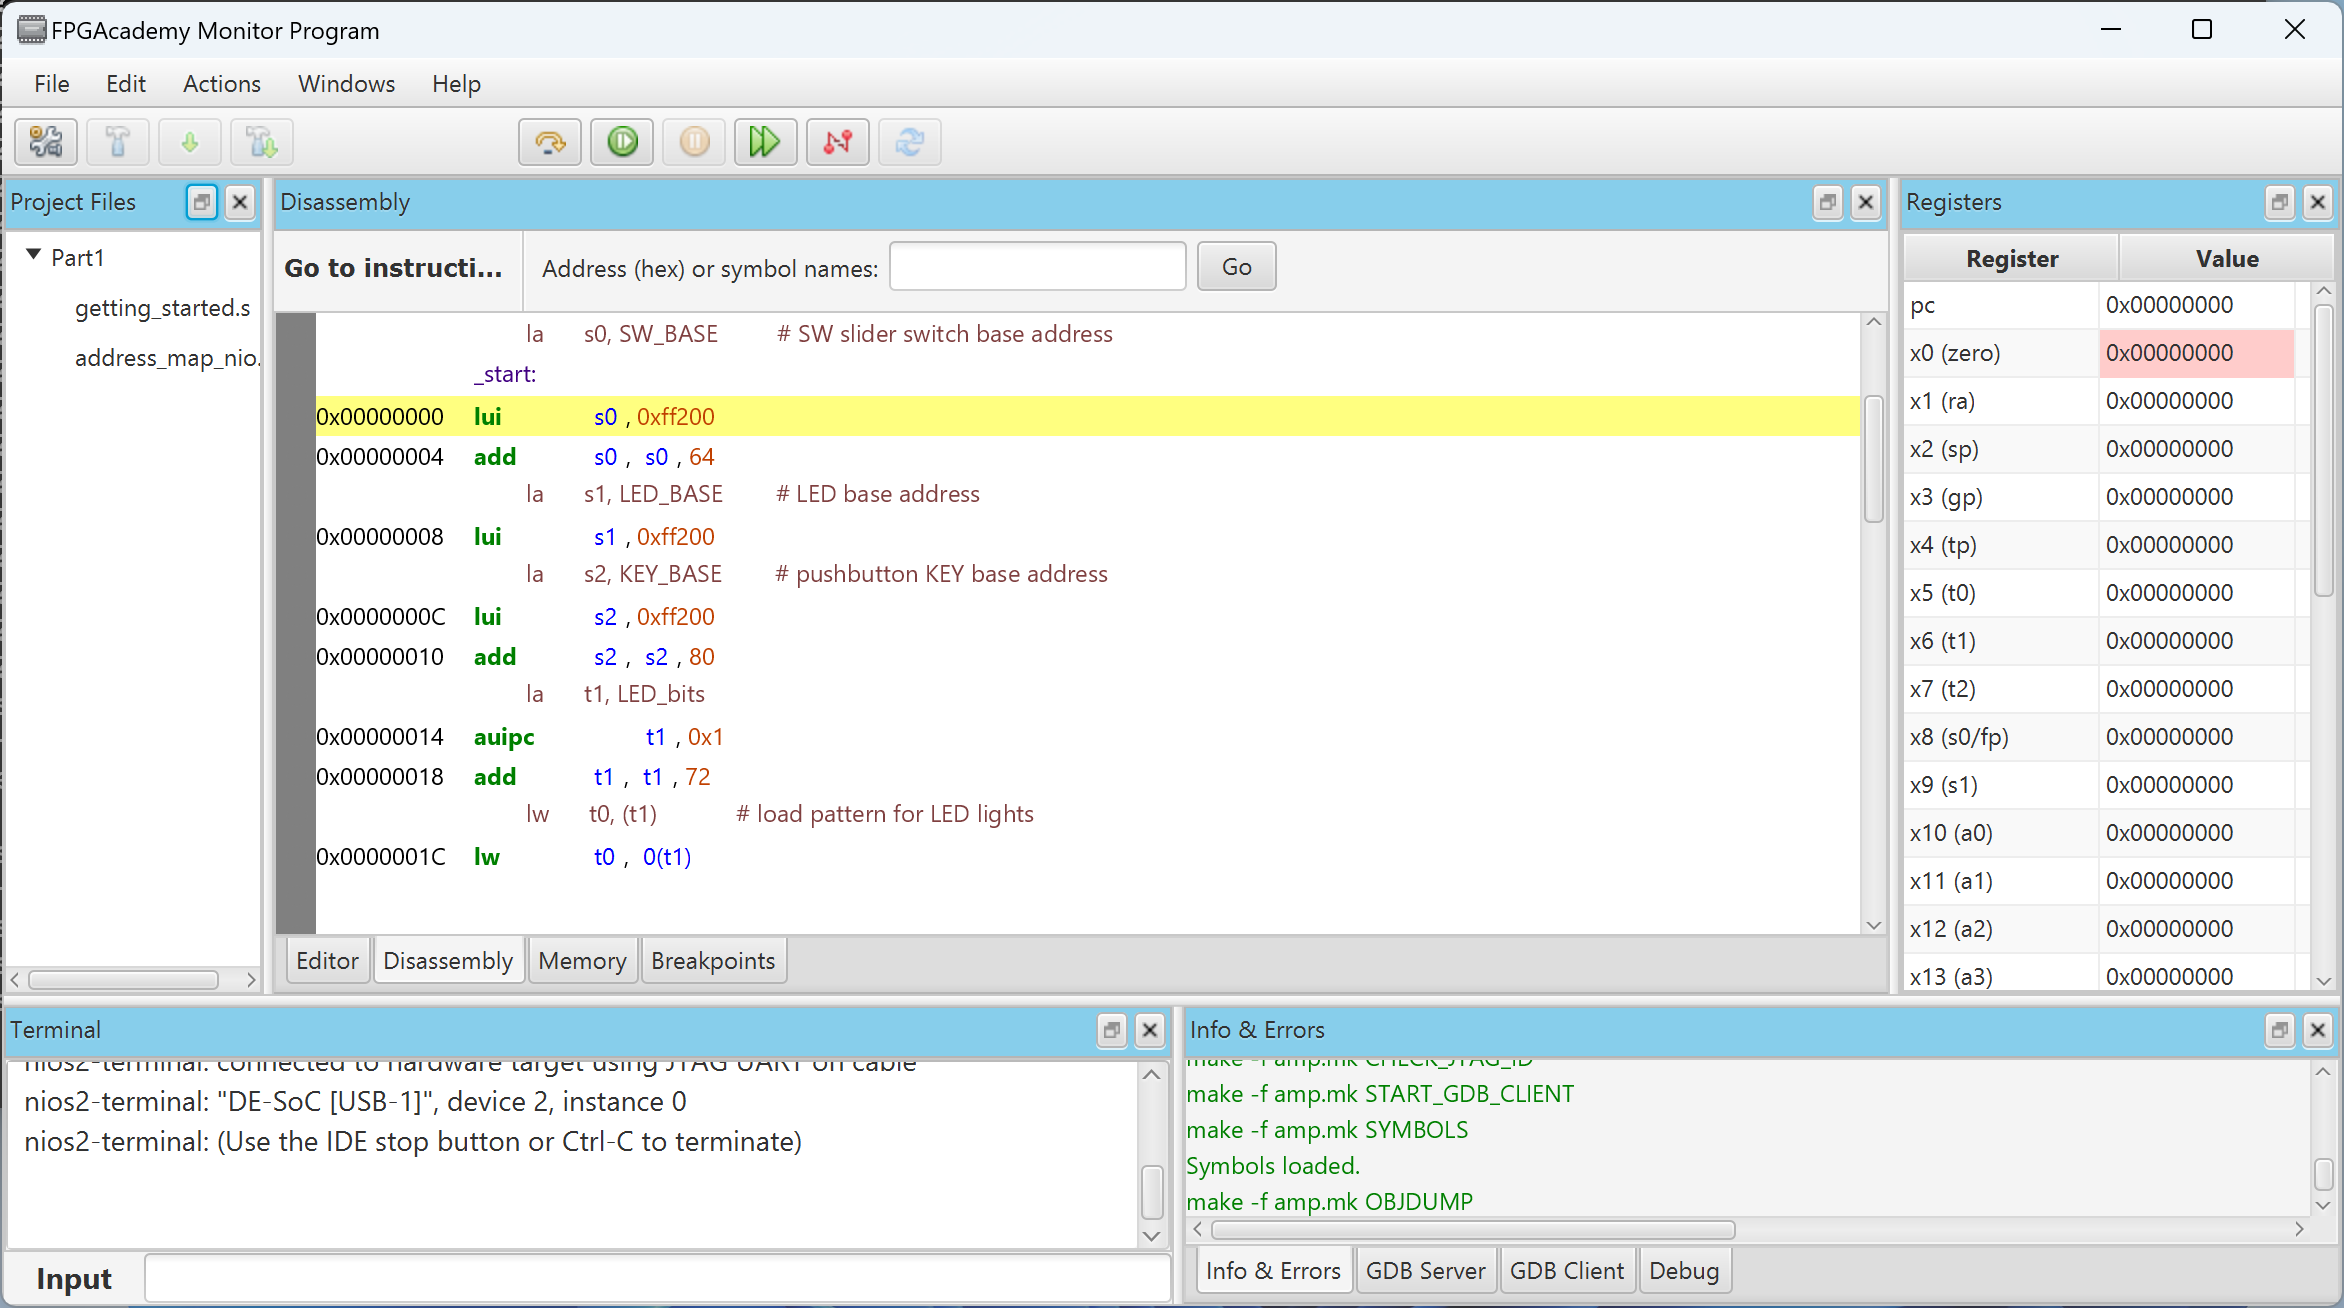
\includegraphics[scale=0.33]{figures/Snap11.png}
	\end{center}
	\caption{The monitor window showing the loaded sample program.}
\label{fig:MP9}
\end{figure}

\end{enumerate}

\subsection*{Part VII}
~\\
~\\
\noindent
Now, we will explore some features of the Monitor Program by using the Nios~V
assembly-language code from Part II, which finds the largest number in a 
list of 32-bit integers that is stored in the memory. For convenience, the code is reproduced 
in Figure~\ref{fig:code_repeat}.

\begin{figure}[H]
\begin{center}
\lstinputlisting[style=defaultNiosVStyle]{../design_files/part2.s}
\end{center}
\caption{Assembly-language program that finds the largest number.}
\label{fig:code_repeat}
\end{figure}

~\\
\noindent
Perform the following:

\begin{enumerate}
\item Create a new folder for this part of the exercise, with a name such as {\it Part2}.  
Create a file named {\it part2.s} and enter the code from Figure~\ref{fig:code_repeat} into this
file.  Use the Monitor Program to create a new project in this folder; we have chosen the 
project name {\it part2}.  When you reach the window in Figure~\ref{fig:MP4} 
choose {\sf Assembly Program} but do not select a sample program. Click {\sf Next}.
\item Upon reaching the window in Figure~\ref{fig:MP5}, you have to specify the source
code file for your program. Click {\sf Add} and in the pop-up box that appears 
indicate the desired file name,
{\it part2.s}.  Click {\sf Next} to get to the window in Figure~\ref{fig:MP6}. 
Again click {\sf Next} to get to the window in Figure~\ref{fig:MP7}. Notice that the 
SDRAM is selected as the memory device.  Your program will be loaded starting at
address 0 in this memory.  Click {\sf Save}. Note that you do not need to download 
the DE1-SoC Computer system to your board, as you already programmed the FPGA chip when
performing Part VI.

\item Compile and load the program. The
Monitor Program will display a disassembled view of the machine code loaded
in the memory, as indicated in Figure~\ref{fig:MP11}. 

\item Execute the program.
When the code is running, you will not be able to see any changes
(such as the contents of registers or memory locations) in the display for the Monitor Program,
because it does not communicate with the Nios~V processor while code is being
executed.  But, if you pause the program then the Monitor Program window will be updated.
Pause the program 
and observe that the processor stops within the endless loop {\bf stop: j stop}.
Note that the largest number found in the sample list is 8 as indicated
by the contents of register {\it t3}. This result is also stored in memory at the label
{\it result}.  The address of the label {\it result} for this program in the Monitor
Program is {\sf 0x00000038}.
Use the Monitor Program's \texttt{Memory} tab, as illustrated in Figure~\ref{fig:MP_mem},
to verify that the resulting value 8 is stored in the correct location.

\item You can return control of the program to the start by clicking on the icon 
\hbox{
\includegraphics[scale=0.4]{figures/Restart.png}}, or by selecting 
{\sf Actions} $>$ {\sf Restart}. 
Do this and then single-step through the program by clicking on the icon
\hbox{
\includegraphics[scale=0.4]{figures/Step.png}}. Watch how the instructions change the 
data in the processor's registers.

\item Double-click on the {\sf pc} register in the Monitor Program and then set the program
counter to 0. This action has the same effect as
clicking on the restart icon \hbox{\includegraphics[scale=0.4]{figures/restart.png}}. 

\item Now set a breakpoint at address {\sf 0x0000002C} by clicking on the gray bar to
the left of this address, as illustrated in Figure~\ref{fig:MP13}. Restart the program and run 
it again.  Observe the contents of register {\it t3} each time the instruction at the
breakpoint, which is \texttt{j loop}, is reached.

\begin{figure}[H]
	\begin{center}
	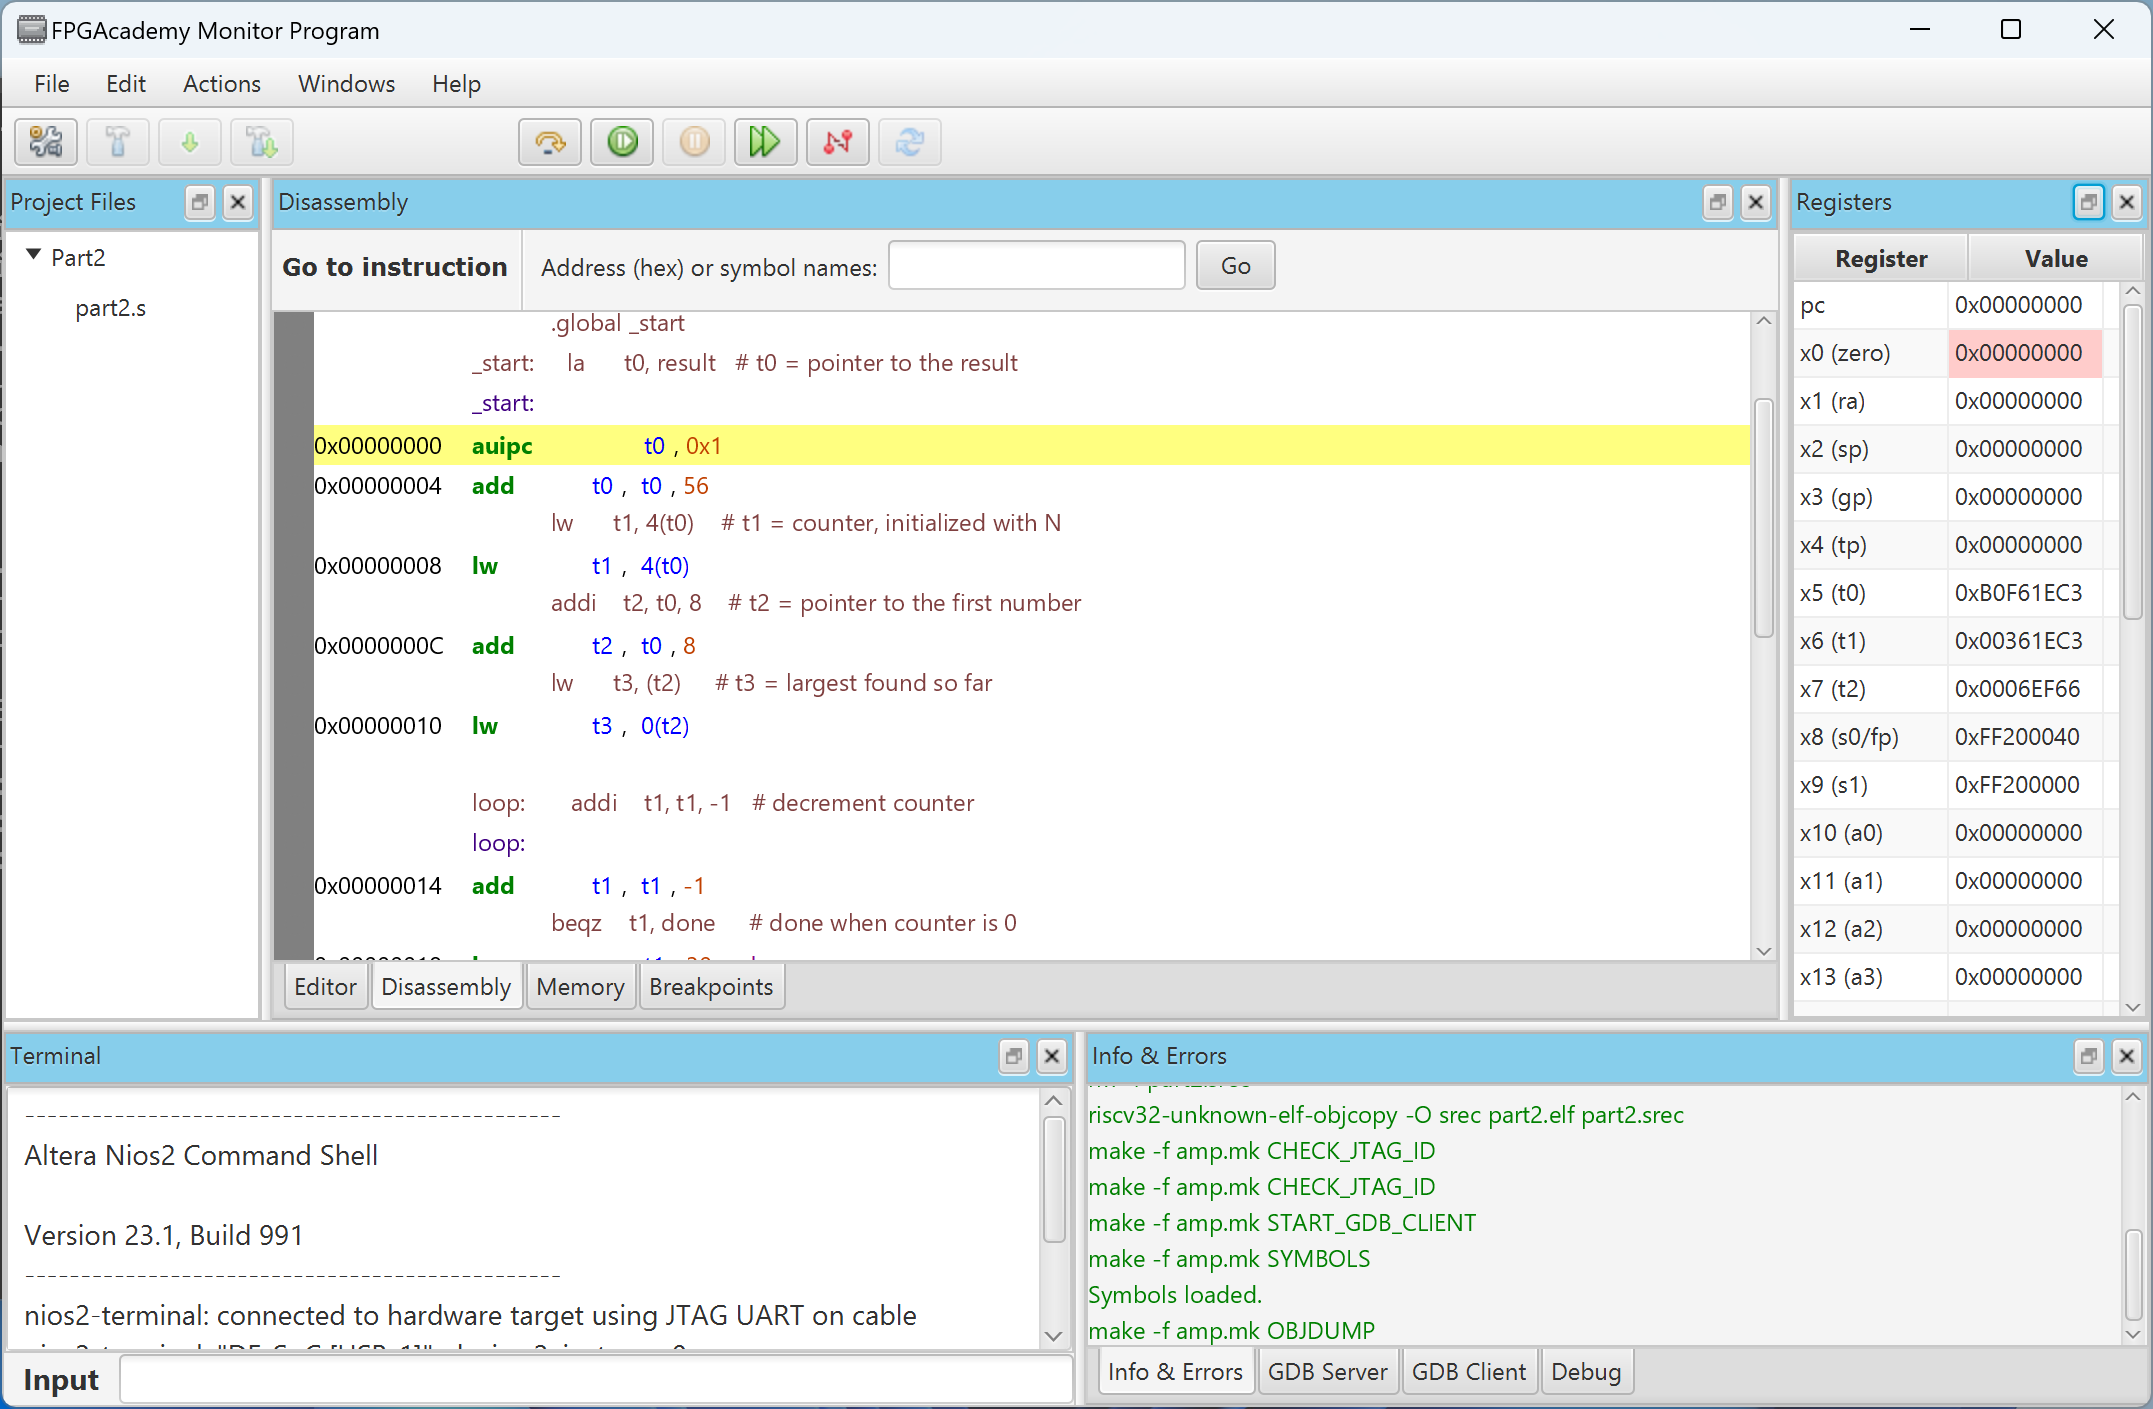
\includegraphics[scale=0.33]{figures/Part2.png}
	\end{center}
	\caption{The disassembled view of the program in Figure~\ref{fig:code}.}
\label{fig:MP11}
\end{figure}

~\\
~\\
{\bf Final Comments}

~\\
\noindent
You may also want to implement the Nios~V programs from Parts III to V, to gain more
experience with the Monitor Program application.

~\\
\noindent
In this exercise we
have provided only a brief introduction to the features of the Monitor Program
application software. A more detailed discussion is 
available in the tutorial {\it Monitor Program Tutorial for the Nios~V Processor}, 
which is available as part of the 
\texttt{Computer Organization System Design} tutorials (version 23.1) on
{\small \href{https://www.fpgacademy.org/tutorials.html} {FPGAcademy.org}}.
This tutorial may also be available within the Monitor Program itself via the command
{\sf Help $>$ Tutorial}.

\begin{figure}[H]
	\begin{center}
	\includegraphics[scale=0.3]{figures/memory.png}
	\end{center}
	\vspace{-0.5cm}\caption{Displaying the result in the memory tab.}
\label{fig:MP_mem}
\end{figure} 

\begin{figure}[H]
	\begin{center}
	\includegraphics[scale=0.3]{figures/break.png}
	\end{center}
	\vspace{-0.5cm}\caption{Setting a breakpoint.}
\label{fig:MP13}
\end{figure} 

\end{enumerate}

\input{\CommonDocsPath/copyright.tex}
\end{document}
\end{document}
